
\documentclass[conference,compsoc]{IEEEtran}

\usepackage{amsmath,amssymb,amsfonts,amsthm}
\usepackage{graphicx}
\graphicspath{{figures/}{./}}
\usepackage{booktabs}
\usepackage{multirow}
\usepackage{placeins}
\usepackage{stfloats}
\usepackage{threeparttable}
\usepackage{tabularx}
\usepackage{array}
\usepackage{enumerate}
\usepackage{siunitx}

\usepackage{pifont}
\newcommand{\cmark}{\ding{51}}  
\newcommand{\xmark}{\ding{55}}  
\newcommand{\biophoto}[1]{
  \IfFileExists{#1}{\includegraphics[width=1in,height=1.25in,clip,keepaspectratio]{#1}}{}
}
\newcolumntype{Y}{>{\raggedright\arraybackslash}X}

\usepackage{soul}
\usepackage{url}
\usepackage[table]{xcolor}

\theoremstyle{definition}
\ifdefined\SUPPLEMENTDOC
  
  
  
  \newtheorem{definition}{Definition}[section]
  \newtheorem{challenge}{Challenge}[section]
  \newtheorem{assumption}{Assumption}[section]
\else
  \newtheorem{definition}{Definition}
  \newtheorem{challenge}{Challenge}
  \newtheorem{assumption}{Assumption}
\fi
\usepackage{csquotes}
\usepackage[
  backend=biber,
  style=ieee,
  citestyle=numeric-comp,
  sorting=none,
  sortcites=true,
  doi=false,
  url=false,
  maxbibnames=6,
  minbibnames=1
]{biblatex}

\addbibresource{reference.bib}

\usepackage[hidelinks]{hyperref}
\usepackage{xr-hyper}
\ifdefined\SUPPLEMENTDOC
  \hypersetup{
    pdftitle={Supplemental Material for Closing the History-to-Release Gap in Stateful Private Aggregation},
    pdfauthor={},
    pdfsubject={Appendix to the main paper},
    pdfkeywords={supplemental material, stateful private heatmap aggregation, zero-knowledge proofs}
  }
  
  
  
  \numberwithin{equation}{section}
  \numberwithin{table}{section}
  \numberwithin{figure}{section}
\else
  \hypersetup{
    pdftitle={Enforcing Hidden-State Policies in Native Private Aggregation},
    pdfauthor={},
    pdfsubject={Hidden-state authorization bound to retained native outputs and complete first exposure},
    pdfkeywords={private aggregation, stateful authorization, semantic binding, release integrity, SHTPC}
  }
  
  
  
\fi
\theoremstyle{plain}
\ifdefined\SUPPLEMENTDOC
  \newtheorem{theorem}{Theorem}[section]
  \newtheorem{lemma}{Lemma}[section]
  \newtheorem{corollary}{Corollary}[section]
  \newtheorem{proposition}{Proposition}[section]
\else
  \newtheorem{theorem}{Theorem}
  \newtheorem{lemma}{Lemma}
  \newtheorem{corollary}{Corollary}
  \newtheorem{proposition}{Proposition}
\fi

\pagestyle{plain}

\hyphenation{op-tical net-works semi-conduc-tor}


\newcommand{\VFourConstraints}{9{,}726}
\newcommand{\VFourPublicInputs}{23}
\newcommand{\VFourPrivateInputs}{25}
\newcommand{\VFourStaticChecks}{35}
\newcommand{\VFourProtocolDatasets}{1}




\newcommand{\ShareRingBits}{32}
\newcommand{\BnFieldBits}{254}

\usepackage{tikz}
\usetikzlibrary{arrows.meta,shapes.geometric,calc}
\begin{document}
\title{Enforcing Hidden-State Policies in Native Private Aggregation}
\author{}
\maketitle
\begin{abstract}
A managed fleet task can aggregate reports from a complete predeclared cohort
while keeping client state hidden from the admission authority. A malicious report that
moves a contribution to another cell, or the omission of an accepted report,
can distort the resulting heatmap even when every aggregated input is individually
valid. These attacks change a payload relative to an authorized claim. A fabricated
but policy-conformant claimed trajectory remains outside the physical-truth
guarantee. The aggregate therefore needs to reflect the transitions authorized against
each client's hidden history. Stateful History-to-Payload Closure (SHTPC)
connects those transitions to the outputs retained by Prio3 and to the complete
cohort exposed at release. Its masked moment uses native one-hot validity to
bind the authorized cell without reproducing native seed expansion in the
application circuit. The standalone binding relation has 5,779 constraints at
each evaluated histogram size, while native processing still scans the vector.
Atomic admission advances the history, and durable reservation fixes the cohort
before an honest aggregate share becomes decryptable. With correctly executing
services, the integrity analysis covers accepted history across windows and
first exposure. A separate privacy analysis covers one complete cohort per
task and key against an active aggregator colluding with the Collector. It
compares legal histories with common public metadata and equal declared cohort
sums. Janus tests reject native-valid mismatches, block a distinguishing
subset exposure and recover exact 100-member outputs after withheld deliveries.
\end{abstract}
\section{Introduction}
\label{sec:intro}

A fleet operator uses a heatmap to identify congestion and allocate vehicles,
while drivers keep their locations private. Private location statistics and
accountable vehicular services motivate this combination of confidentiality
and admissible contributions~\cite{Popa2011PrivStats,Popa2009VPriv,Balasch2010PrETP}.
If a participant redirects a
report from its authorized cell to a target cell, the target count rises and
the original count falls. A dispatcher can then act on a hotspot that the
authorized reports do not support. Omitting an accepted report can similarly
hide demand. These errors concern the meaning and membership of the aggregate,
even when the aggregation arithmetic is correct.

In a controlled offline replay of 100 selected T-Drive histories, redirecting
20 reports to the clean modal cell raises its count from 3 to 22--23 across
three fixed actor permutations. An exact-set release contract then withholds
the window if substituted contributions remain unresolved. Section~\ref{sec:eval-real-traces}
examines this integrity and availability tradeoff with the selection losses
of the real trajectories.

Periodic reporting motivates complete cohorts when a missing accepted report
can distort a decision. The integrity contract supports continued accepted
history across windows, including after abort. The privacy theorem covers one
visible complete cohort per task and key, not the composition of multiple
outputs, even from nonoverlapping windows. An admission authority authorizes transitions and records
quotas without reading client coordinates. Two aggregation roles process
secret shares, and a Collector consumes statistics for a fixed
cohort. DAP with
Prio3~\cite{Geoghegan2026DAP,Barnes2023VDAF08,Corrigan2017Prio} provides
native validation and private aggregation. The managed services enforce the
integrity contract, while clients and transport may be malicious. The
application needs the authorized transitions, retained contributions and
release membership to describe the same accepted history.

Existing protocols validate private inputs~\cite{Bell2023ACORN,Chowdhury2022EIFFeL,Rathee2023ELSA,Lycklama2023RoFL},
enforce inclusion or verify aggregates~\cite{Su2025SCIF,Acharya2025PEAR,Hahn2023VerSA},
and maintain private aggregate state~\cite{Ball2024Stateful}.
The application here needs these interfaces to refer to one accepted history.
Consider a proof that authorizes cell \(p\) and a native-valid report that
encodes cell \(q\ne p\). Both objects pass their respective checks even when
they share a report identifier and a signed body. The identifier authenticates
their association, not their semantic equality. A hiding commitment likewise
binds its committed value without proving that this value determines the
native output. The missing relation connects the hidden witness to the output
actually retained for aggregation. A generic commitment scheme that proves
this equality would close this particular gap.

State freshness and release membership create two further interfaces. A proof
for predecessor \(c\) remains valid after a competing successor commits, so
proof verification does not authorize the current transition. Separately, an
accepted report can be dropped on both receiver channels. The receivers then
agree on a valid but incomplete batch, as Figure~\ref{fig:gap} shows. These
failures break the same connection between the history authorized by the
application, the values aggregated and the cohort exposed to the Collector.

\begin{figure}[t]
\centering
\begin{tikzpicture}[
  font=\footnotesize, >={Stealth[length=4pt]},
  box/.style={draw, rounded corners=2pt, align=center, inner sep=3pt,
              minimum height=7mm},
  lost/.style={densely dashed, red!70!black}]
  \node[box] (cl) at (0,0)       {Clients\\\(r_0,\ r_1\)};
  \node[box] (ad) at (0,1.6)     {Admission\\\(\mathcal A_w=\{r_0,r_1\}\)};
  \node[box] (le) at (3.1,0.8)   {Leader\\\(B=\{r_0\}\)};
  \node[box] (he) at (3.1,-0.8)  {Helper\\\(B=\{r_0\}\)};
  \node[box] (co) at (6.0,0)     {Collector\\count, checksum\\agree, release \(m_0\)};
  \draw[->] (cl) -- (ad) node[midway, right] {accept};
  \draw[->] (cl.east) -- node[above, sloped, pos=0.75] {\(r_0\)} (le.west);
  \draw[->] (cl.east) -- node[below, sloped, pos=0.75] {\(r_0\)} (he.west);
  \draw[lost] (cl.east) -- ++(0.75,0) coordinate (x);
  \draw[red!70!black, thick] ($(x)+(-0.07,-0.07)$) -- ($(x)+(0.07,0.07)$)
                             ($(x)+(-0.07,0.07)$) -- ($(x)+(0.07,-0.07)$);
  \node[red!70!black, font=\scriptsize, anchor=west] at ($(x)+(0.1,0)$)
    {\(r_1\) lost};
  \draw[->] (le.east) -- ([yshift=5pt]co.west);
  \draw[->] (he.east) -- ([yshift=-5pt]co.west);
  \draw[->, densely dotted] (ad.east) -| node[pos=0.25, above]
    {expected \(m_0+m_1\)} (co.north);
\end{tikzpicture}
\caption{Both aggregators can agree on a batch that omits an accepted report.}
\label{fig:gap}
\end{figure}

Completeness also has a privacy deadline. Two legal histories can have
identical complete heatmaps but different subset aggregates. A final
publication check can refuse an incomplete cohort, but it cannot retract an
aggregate share that already exposed the subset. Accepted-history closure
therefore connects each admitted claim to its consumed payload and atomic
state transition. It also reconciles the complete eligible set before the
first honest share becomes decryptable.

Stateful History-to-Payload Closure (SHTPC) realizes the payload connection
without reproducing native seed expansion inside the application circuit.
Prio3Histogram validity restricts the reconstructed contribution to a one-hot
vector with a sentinel. On that domain, the linear index moment identifies
the selected cell. Each role computes a masked receipt from the output it
actually retained, and admission checks the receipts against the hidden-state
proof. The binding relation is independent of histogram width, although
native vector processing remains \(O(D)\).

This bridge introduces receipts and retry feedback that neither component's
isolated analysis covers. Authenticated source registration isolates the
hidden input, while joint simulation couples receipts, errors, aborts and
retries to the native transcript. Atomic admission rechecks the actual head,
anchor and quota before commit. Each role applies authorized decisions once
and durably reserves the complete eligible sum before sending its share.
Figures~\ref{fig:architecture} and~\ref{fig:accepted-history-flow} show these
boundaries and their execution order. Integrity assumes correct services.
Privacy separately permits one actively corrupted aggregator colluding with
the Collector under declared metadata and equal complete-cohort aggregates.

\begin{figure*}[t]
\centering
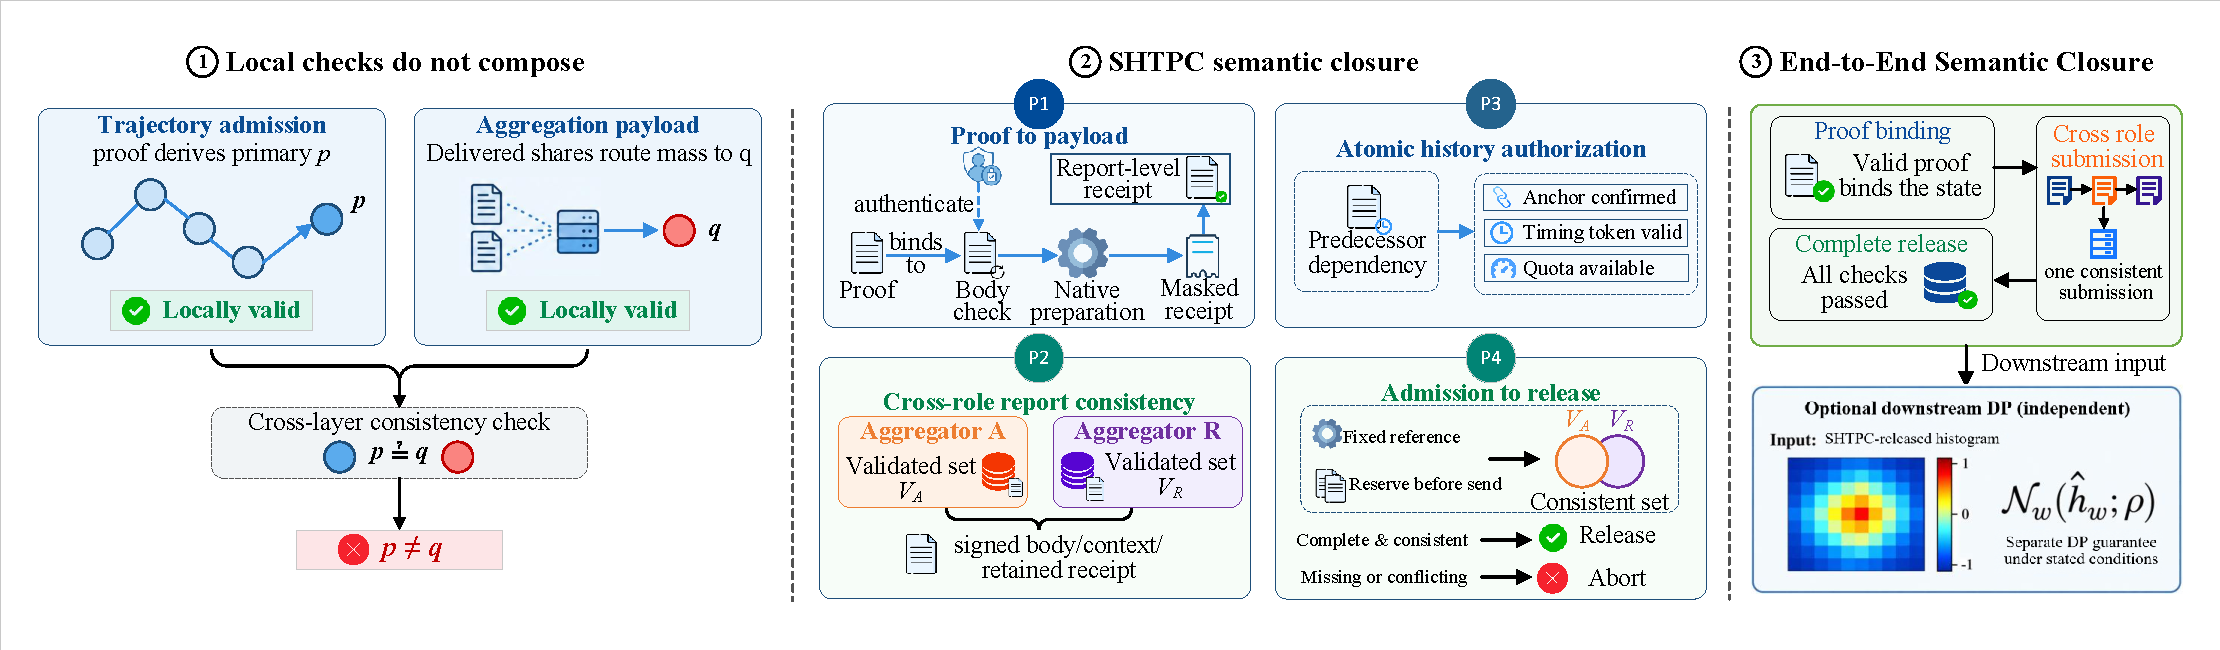
\includegraphics[width=\textwidth]{figures/overview_1.pdf}
\caption{SHTPC connects report meaning, accepted history and complete release through four semantic boundaries.}
\label{fig:architecture}
\end{figure*}

The central contribution is the composition of an accepted-history contract,
native-output binding, source and feedback protection, and reservation before
first exposure. The contributions are as follows.
\begin{enumerate}
\item \emph{Accepted-history contract.} A security contract connects hidden
claims, actual native outputs, legal state advancement and complete membership
at first exposure. Separating executions identify the missing semantic,
history and exposure information.
\item \emph{Compact native-output binding.} A masked-moment adaptor uses
Prio3Histogram validity to connect hidden state proofs to retained outputs.
Its binding relation is independent of histogram width and leaves native seed
expansion outside the circuit.
\item \emph{Privacy and recovery composition.} Source isolation and joint
simulation account for receipt feedback. Under their respective models, the
analysis establishes observer privacy and history closure across atomic
admission, durable reservation and retries.
\item \emph{Native realization and evidence.} A Janus implementation exercises
semantic substitution, source-feedback and subset-exposure controls together
with durable recovery. Materialized circuits and mechanism-level measurements
characterize computational costs.
\end{enumerate}

Section~\ref{sec:prelim} defines the contract, Section~\ref{sec:system}
presents the construction and Sections~\ref{sec:security-summary}
and~\ref{sec:evaluation} give its analysis and evaluation. Related work,
limitations and artifact information follow.

\section{Model and Security Contract}
\label{sec:prelim}

This section defines the deployment, accepted histories and release contract.
\subsection{Deployment and Trust Model}
\label{sec:threat}

Enrolled clients report under stable pseudonymous identities. An admission
authority verifies hidden state proofs and maintains accepted history without
receiving coordinate openings or role decryption keys. Two Aggregators prepare
and retain Prio3 outputs. The Collector holds the aggregate-share HPKE key,
and its Decoder verifies release records and reconstructs the heatmap. The
authority-side Finalizer authenticates the frozen reference and its completion.
Its certificate joins that reference to both roles' matching attestations
rather than introducing another trust anchor. A durable admission proxy
belongs to the same trust domain and delivers signed decisions. Each role
durably reserves its own share before export.

Integrity and privacy use separate corruption models. For integrity, clients
and transport are malicious, while admission, both Aggregators, Finalizer,
Collector and Decoder execute the protocol. This model fits a managed domain
whose operator enforces admission and release rules against deviating clients
and unreliable transport. Serialized durable storage preserves committed
history, retained outputs and reservations across recovery. Correct service
execution does not give the authority coordinate openings. For privacy, one
Aggregator may be actively corrupted with the
Collector. The authority, honest clients, Finalizer and Decoder follow the
protocol. The observer may also receive the correct authority's business records,
receipts, diagnostics and backups. Sharing does
not transfer its signing key or authorize malicious issuance. A corrupted
role can fabricate shares or abort, so this model makes no output-integrity
claim. Corrupt admission is outside both guarantees.

Privacy challenges use legal histories with common public structure \(\mu\),
including identities, task and key, windows, step and anchor references,
eligibility, contribution bits, packet rules and the delivery plan. Proofs,
ciphertexts, commitments, receipts, errors, aborts and retries are simulated
jointly. The authority has no aggregate interface. The aggregation observer
has one visible cohort per task and key, with equal declared native-index sums
on that complete cohort. Definition~\ref{game:privacy} specifies the views and
the first-exposure interface. Activity, contribution bits and cadence remain public. The permitted
exact aggregate can itself support inference from auxiliary knowledge. The
claim bounds additional protocol leakage rather than inference from that
output and \(\mu\). It does not establish privacy for multiple outputs, including nonoverlapping
windows, or hide network traffic beyond \(\mu\).

Correctly sampled setup with unknown trapdoors, reviewed fixed-width
arithmetic, authenticated confidential registration and the declared durable
execution boundaries are premises. Enrollment authenticates identity rather
than physical location or Sybil resistance. Continuity uses authenticated
slots rather than unverified elapsed time. No transparency mechanism detects
authority equivocation in this model.

\subsection{Reports, Histories and Cohorts}
\label{sec:prelim-model}

A sampling slot assigns a measurement to time, an accepted step counts a
committed transition, and a release window groups eligible reports. Rejected
attempts do not advance accepted history.

Each report is projected and quantized under fixed public parameters, yielding
a hidden vector \(\mathbf{x}_r\). A \(W\times H\) grid with cell width \(s\)
selects
\begin{equation}
  p_r=\mathsf{Grid}(\mathbf{x}_r)
  =W\Bigl\lfloor\frac{y_r}{s}\Bigr\rfloor+\Bigl\lfloor\frac{x_r}{s}\Bigr\rfloor,
  \label{eq:canonical-grid}
\end{equation}
where \(D=WH\). The evaluated profile uses \(s=100\) and \(W=H=100\).
The replay projection, rounding and boundary rules appear in
Appendix~\ref{app:policy}.

Consider two drivers whose reports are registered for the same window. The
candidate map \(P_w\) fixes their registered core records before preparation
feedback, and \(R_w=\mathsf{eligible}(P_w)\) selects the eligible cores. A
committed record extends its core with authenticated receipts, decision and
retained-output links. Projection \(\pi_{\rm reg}\) removes those later fields. Admission records committed transitions in \(L_w\), whose
eligible projection is \(\mathcal A_w=\mathsf{eligible}(L_w)\). Each role's
map \(M_{S,w}\) records the eligible decisions it has applied. If one
delivery is delayed, the role's map is incomplete even though its local native
batch is valid. Release compares that map with the fixed \(R_w\), rather than
using the local batch as the cohort.

Warmups enter the log but not the eligible maps. Eligible zero-bit records
remain members despite adding no mass. Credential epochs and storage revisions
do not replace accepted-step counters or sampling slots.

For report \(r\), the common admitted object is
\begin{equation}
  A_r=(\mathsf{rid}_r,\eta_r,\mathsf{stmt}_r,\mathsf{pay}_r,
       c_{r-1},c_r,w,b_r).
  \label{eq:admission-object}
\end{equation}
The context \(\eta_r\) binds identity, window and policy. The remaining fields
identify the proof statement, bound channel packages, predecessor, successor
and contribution bit. A complete signed body, two retained-output receipts and
one commit decision authenticate this object in the native realization
(Appendix~\ref{app:native-theory}).

Strict release produces the complete eligible cohort or refuses. The native
prototype uses a finite preconfigured schedule, not a roster selected from
arrivals. Table~\ref{tab:lifecycle} gives its window lifecycle.

\begin{table}[t]
\centering
\caption{Native window lifecycle and scope.}
\label{tab:lifecycle}
\footnotesize
\begin{tabularx}{\columnwidth}{@{}lY@{}}
\toprule
Stage & Contract \\
\midrule
Register & All predeclared UID and contiguous step slots, including warmups and eligible zeros, need full pending bodies. \\
Lock & At the registration boundary, the complete graph starts at actual heads. Both roles install the lock. \\
Process & Current-head permits precede preparation and commit. Both roles apply decisions. \\
Expose & Complete records are reserved before the first share. Retries use the same snapshot. \\
Abort & Partial commits and quota persist. Later configured slots and new bodies start at actual heads. \\
\bottomrule
\end{tabularx}
\end{table}

After an abort leaves two owners at steps 2 and 1, their next configured
slots start at 3 and 2 with new bodies referencing those heads. An incompatible
schedule cannot lock. Configuration remains bound to the database. This
integrity continuation does not extend the single-cohort privacy experiment.

\subsection{Accepted-History Closure}
\label{sec:boundaries}
\label{sec:prelim-goals}
\label{sec:composition-summary}

Four obligations share \(A_r\). P1 connects the proved claim to the consumed
package by
\begin{equation}
\mathsf{Contrib}(\mathsf{pay}_{r,\mathrm{consumed}})
  =b_r\mathbf e_{p_r}.
  \label{eq:p1}
\end{equation}
P2 requires both roles to consume channels of that same object. P3 gives each
accepted object one atomic transition with its quota charge.
\begin{equation}
  \mathrm{State}_{r-1}\rightarrow\mathrm{State}_{r}
  \label{eq:p3}
\end{equation}
P4 requires a successful release to contain exactly the eligible committed
records and the complete locked reference.
\begin{equation}
  \pi_{\rm reg}(\mathcal A_w)=R_w .
  \label{eq:p4}
\end{equation}
Together these obligations express accepted-history closure.
\begin{equation}
  \mathrm{P1}\land\mathrm{P2}\land\mathrm{P3}\land\mathrm{P4}
  \;\Rightarrow\;\text{Accepted-History Closure}.
  \label{eq:closure}
\end{equation}

\begin{definition}[Legal sequential history]
\label{def:legal-history}
A sequence \(H=(A_1,\ldots,A_n)\) with unique identifiers is legal if replay
from enrolled genesis enables every transition. Each step has an authorized
owner and context, names the current head and policy-selected accepted anchor,
and satisfies the application relation on opened states. It atomically appends
the successor, advances the head and accepted-step counter, and charges quota
without changing other owners. Rejected and uncommitted attempts add no step.
\end{definition}

\begin{definition}[History refinement]
\label{def:history-refinement}
For a finite prefix, \(\mathcal L\preceq H\) when committed admission
operations bijectively map to a legal \(H\), preserving every \(A_r\) field
and the order of linearization points between invocation and response.
Committed pending operations are completed at the prefix end, while
uncommitted attempts are discarded. Retries of one durable decision represent
one operation, and distinct committed effects remain distinct.
\end{definition}

\begin{definition}[Successful-trace closure]
\label{def:trace-closure}
Fix a transition policy, additive contribution map \(r\mapsto m_r\) and
eligibility rule. A successful release has closure if some legal \(H\)
satisfies \(\mathcal L\preceq H\). Let \(E_w(H)\) be the set of records in
the complete accepted history \(H\) that belong to window \(w\) and satisfy
the eligibility rule. Their identifiers equal \(\operatorname{dom}(\mathcal A_w)\),
and each identifies one common admitted object across proof, packages,
transition and certificate. Each role has
\(N_{S,w}(r)=\mathbf1[r\in\operatorname{dom}(\mathcal A_w)]\), and its reserved sum uses exactly
those retained outputs. The pre-noise output is
\(\sum_{r\in\operatorname{dom}(\mathcal A_w)}m_r\). For heatmaps,
\(m_r=b_r\mathbf e_{\mathsf{Grid}(\mathbf x_r)}\). Eligibility is independent
of bit value. These are policy-consistent admitted claims rather than verified
physical locations.
\end{definition}

\begin{definition}[Exposure-prefix safety]
\label{def:exposure-prefix}
Every decryptable honest share comes from a prior durable reservation
satisfying
\begin{equation}
 \begin{gathered}
 \pi_{\rm reg}(L_{S,w})=P_w,\qquad
 \pi_{\rm reg}(M_{S,w})=R_w=\pi_{\rm reg}(\mathcal A_w),\\
 \mathbf a_{S,w}=\sum_{r\in R_w}v_{S,r}.
 \end{gathered}
 \label{eq:export-safety}
\end{equation}
Retries preserve its membership and plaintext. Successful-trace closure also
requires correct final reconstruction.
\end{definition}

Independent local checks do not supply these relations. For fixed context
\(\eta\), let \(\mathcal A_p^\eta\) and \(\mathcal G_p^\eta\) contain
application and payload objects with primary \(p\).
\begin{proposition}[Role-separability observation]
\label{prop:rectangularity-main}
Independent acceptance is a Cartesian product. The same-primary relation
\(\bigcup_p\mathcal A_p^\eta\times\mathcal G_p^\eta\) is not a product
when two primaries are feasible on both sides.
\end{proposition}
The observation identifies the missing correlation rather than ruling out a
shared tag or joint relation~\cite{Kushilevitz1997Communication}.
Appendix~\ref{sec:composition-failures} gives the short proof.

\begin{proposition}[History and release separation]
\label{thm:interface-separation-main}
\label{sec:interface-necessity}
A proof for predecessor \(c\) remains valid after a competing successor
commits. Receivers seeing only \(R\) also cannot distinguish accepted set
\(R\) from \(R\cup\{r^\star\}\) when \(r^\star\) is dropped on both channels.
Checks on those identical views cannot accept the complete case and reject
the incomplete one.
\end{proposition}
Current-head evidence and an authenticated complete-set reference supply the
missing history-dependent information without fixing a database or proof
format. Appendix~\ref{sec:history-interface} formalizes the views.

\section{SHTPC Design}
\label{sec:system}

This section describes how SHTPC realizes P1--P4 in a native Prio3 workflow.
\subsection{Design Overview}
\label{sec:architecture-choice}
\label{sec:overview}

Figure~\ref{fig:accepted-history-flow} follows one report from registration
to exposure. The client proves Anchor Distance Window Continuity (ADWC) and
grid membership over hidden states. Admission locks the registered graph before
private preparation, checks both retained-output receipts, and commits against
the current history. A durable proxy delivers that decision for exactly-once
application. Each role reserves the complete eligible sum before sending its
share. Preparation creates a retained output, while admission authorizes its
use in aggregation.

\begin{figure}[t]
\centering

\begin{tikzpicture}[
  x=1cm,y=1cm,font=\small,>={Latex[length=4pt]},
  line/.style={->,draw=black!65,line width=.65pt},
  plain/.style={draw=black!65,line width=.65pt},
  box/.style={draw=black!45,rounded corners=3pt,line width=.65pt,
    align=center,inner xsep=4pt,inner ysep=5pt},
  note/.style={font=\footnotesize,fill=white,inner sep=2pt},
  authority/.style={box,fill=orange!6,draw=orange!55!black},
  role/.style={box,fill=blue!4,draw=blue!45!black}
]
\node[authority,text width=6.4cm] (register) at (.2,0)
  {Register signed bodies and lock $P_w,R_w$\\
   Before preparation or receipt feedback};
\node[box,text width=6.4cm] (prepare) at (.2,-1.20)
  {Prepare and retain native outputs\\
   Actual-head permit and paired moment receipts};
\node[authority,text width=6.4cm] (accept) at (.2,-2.60)
  {Commit admission atomically\\
   Recheck head, anchor and quota\\
   Persist successor, history and signed decision};
\draw[line] (register) -- (prepare);
\draw[line] (prepare) -- (accept);

\node[role,text width=2.9cm,minimum height=1.30cm] (apply) at (-1.55,-4.35)
  {Each role $S$\\
   Apply decisions once\\
   Update $L_{S,w},M_{S,w}$};
\node[authority,text width=2.9cm,minimum height=1.30cm] (lock) at (1.95,-4.35)
  {Installed lock\\
   Fixed $P_w,R_w$\\
   Before preparation};
\coordinate (fork) at (.2,-3.48);
\draw[plain] (accept.south) -- (fork);
\draw[line] (fork) -| (apply.north);
\draw[line] (fork) -| (lock.north);


\draw[draw=blue!45!black,dashed,rounded corners=4pt,line width=.65pt]
  (-2.02,-5.57) rectangle (3.42,-8.85);
\node[note,text=blue!45!black] at (.7,-5.57)
  {Export transaction};
\node[role,text width=4.7cm] (check) at (.7,-6.30)
  {Complete bound maps?\\
   $\pi_{\rm reg}(L_{S,w})=P_w,\quad \pi_{\rm reg}(M_{S,w})=R_w$};
\coordinate (merge) at (.7,-5.20);
\draw[plain] (apply.south) |- (merge);
\draw[plain] (lock.south) |- (merge);
\draw[line] (merge) -- (check.north);
\node[role,text width=4.7cm] (reserve) at (.7,-7.93)
  {Persist the complete snapshot\\
   $P_w,R_w$, selector and\\
   $\mathbf a_{S,w}=\sum_{r\in R_w}v_{S,r}$};
\draw[line] (check.south) -- node[note,right] {yes} (reserve.north);


\node[box,fill=red!4,draw=red!55!black,text width=1.32cm]
  (refuse) at (-3.35,-6.30)
  {Refuse export\\Keep\\$P_w,R_w$};
\draw[line] (check.west) -- node[note,above] {no} (refuse.east);
\draw[line,dashed,draw=red!55!black,rounded corners=3pt]
  (refuse.north) -- (-3.35,-4.35) -- (apply.west);
\node[note,text=red!55!black] at (-3.35,-5.22) {retry};

\node[box,fill=green!6,draw=green!40!black,text width=4.7cm]
  (send) at (.7,-10.35)
  {Send the reserved share\\
   First honest-share exposure\\
   Retries keep the same snapshot};
\draw[line] (reserve.south) -- node[note,right,align=left]
  {durably\\commit first} (send.north);
\draw[line,dashed,rounded corners=3pt]
  (reserve.east) -- (3.95,-7.93) -- (3.95,-10.35) -- (send.east);
\end{tikzpicture}

\caption{SHTPC reserves the complete eligible history before share exposure.}
\label{fig:accepted-history-flow}
\end{figure}

\subsection{Binding Hidden State to Native Outputs}
\label{sec:native-adaptor}

P1 connects the certified cell to the output actually retained for aggregation.
Generic vector binding proves that retained shares reconstruct the certified
vector. SHTPC instead identifies that vector within the native one-hot domain,
leaving seed expansion outside the application circuit.
Table~\ref{tab:binding-designs} compares these choices.

\begin{table}[t]
\centering
\caption{Binding designs establish different relations under the same release contract.}
\label{tab:binding-designs}
\footnotesize
\begin{tabularx}{\columnwidth}{@{}lYY@{}}
\toprule
Approach & Certified connection & Evidence or remaining work \\
\midrule
Association only & Common report or committed value & No retained-output equality \\
Direct seed binding & Seed expansion and selected vector & Measured R1CS size \\
Generic vector binding & Retained shares equal certified vector & Measured transition cost (this work) \\
Masked moment & Certified index equals retained index & Measured R1CS size and native controls \\
\bottomrule
\end{tabularx}
\end{table}

A direct binding proof could reproduce native sharding inside the application
circuit. SHTPC instead reuses the domain established by native validity.
For example, a three-cell one-hot vector \((0,0,1)\) has index-weighted sum
\(0\cdot0+1\cdot0+2\cdot1=2\). Thus its moment identifies the selected
cell. By linearity, the moments of the roles' retained shares combine to
identify the reconstructed one-hot vector. Arbitrary vectors can share a moment.

The public transition statement contains the relation version, predecessor,
successor and anchor commitments and aliases, mask, ticket and receipt
commitments, key tag, masked index, bit, report identifier and context. Its
witness opens those commitments and gives the coordinates, grid cells,
remainders, masks and carry. The relation binds the payload witness's cell and
remainder to the successor and enforces
\(p=\mathsf{Grid}(\mathbf x_r)\),
\(\|\mathbf x_r-\mathbf x_{\rm prev}\|^2\le\tau_u^2\Delta t_t^2\) and
\(\|\mathbf x_r-\mathbf a_t\|^2\le
\min\{\tau_u^2(\Delta T_t^{(K)})^2,c_{\rm policy}^2\}\).
Here \(\mathbf a_t\) is the policy-selected accepted anchor, \(\tau_u\) is the
speed tier and \(c_{\rm policy}\) is the anchor cap. Admission checks that the
referenced predecessor and anchor are the actual accepted ones. The same grid
and distance constraints apply when \(b=0\). Appendix~\ref{app:policy} gives
the parameters, and the artifact's fixed transition circuit gives the ordered
public-signal interface (Section~\ref{sec:artifact}). In native field \(\mathbb F_q\), use \(D<q\) and
\(D+1\) buckets with sentinel \(D\). A state-derived primary \(p<D\) and
public bit \(b\) authorize \(x=bp+(1-b)D\). Native validity gives
\(v_A+v_R=\mathbf e_y\) for some \(y\in[0,D]\).

The client samples private uniform masks \(r_A,r_R\), commits to their openings
and encrypts one for each role. The proof binds the primary, bit, masks and
completed-package context to
\begin{equation}
 \begin{aligned}
 T   &=x+r_A+r_R\pmod q,\\
 m_S &=\sum_{j=0}^{D}jv_S[j]+r_S.
 \end{aligned}
 \label{eq:native-moment}
\end{equation}
Each correct role computes \(m_S\) from its retained output. Admission checks
report, context and statement identities and accepts the paired receipts only
if \(m_A+m_R=T\). Lemma~\ref{lem:native-moment-fidelity} shows that acceptance forces
\(y=x\), giving \(b\mathbf e_p\) after sentinel removal. Canonical scalars enforce
\(x+r_A+r_R=T+\chi q\) with \(\chi\in\{0,1,2\}\), so the different proof and
native fields cannot wrap the equality (Appendix~\ref{app:native-interface}).
Coordinate openings remain client witnesses. Reused state points preserve their
birth domains and exact accepted references.
Receivers recompute the authenticated package context from the actual bytes.
The authority checks the masked equality without receiving either coordinate
opening or a native role key.

The binding relation is independent of \(D\), while native vector processing
remains \(O(D)\). The adaptor separates preparation from accumulation. Each signed
receipt binds the body, configuration, report, native job, terminal wire step
and retained-session identifier; exact retries preserve output and receipt.
The opaque session tag identifies the local output, while the body and report
context pair the roles around the same admitted object.

\subsection{Protecting the Feedback Interface}
\label{sec:origin-feedback}
\label{sec:cross-role}

Encryption does not authenticate an input's owner. An attacker can transplant
an honest ciphertext and substitute a known mask, causing an honest receipt to
reveal the cell before admission rejects the report. This feedback arises from
the new bridge even when the proof and native protocol are secure in isolation.

SHTPC allocates an owner identifier to one complete signed body and registers
it before private processing. Each ingress authenticates the actual metadata, ciphertexts, sidecars,
installed lock and permit against that body. The implementation stores the full body, and ingress checks its actual
consumed bytes. Both retained sessions and receipts therefore name the same
admitted object, realizing P2.

Recovery retains the same source and native state. The Helper journals its
first protected input and response before sending. Identical retries replay
those bytes, while changed inputs or new jobs cannot reopen that branch. The
Leader's lease and transaction fence permit at most one committed transition.
Uncommitted computation can receive new peer feedback, which the joint privacy
analysis includes explicitly.

\subsection{Atomic History Authorization}
\label{sec:admission}

P3 makes proof validity current at commit. Admission verifies the proof before
the transaction, then atomically rechecks the actual head, anchor and quota and
stores the successor, history and signed decision. Both retained-output checks
precede this linearization point. Preparation, admission and role application
use separate databases connected by that decision and its output links.

For stable identity \(u\), task and window \(w\), durable quota
\(q_{u,w}\in\{0,1\}\) is shared across credential epochs. With accepted round
\(t\) and \(N_{\rm warm}=\max(K,2)\),
\begin{equation}
\begin{aligned}
\gamma_t&=b_t\mathbf1[t>N_{\rm warm}],\\
q_{u,w}+\gamma_t&\le1,\qquad
q_{u,w}\gets q_{u,w}+\gamma_t.
\end{aligned}
\label{eq:window-quota}
\end{equation}
Commit induction gives
\begin{equation}
q_{u,w}=\sum_{\substack{r\in\mathcal A_w\\uid(r)=u}} b_r\le1.
\label{eq:quota-invariant}
\end{equation}
Warmups remain in the transition log without charge. Eligible zero-bit updates
remain members and can advance state after quota is spent.

History is keyed by stable \((\mathsf{task},\mathsf{uid})\), with credential,
revision, window, receipt and budget checks inside the transaction. The proxy
queues exact decisions durably before delivery. Role databases apply each
decision once, including out-of-order delivery. Retries return that decision,
and credential rotation preserves history and spent quota.

\subsection{Complete Exposure and Recovery}
\label{sec:finalization}
\label{sec:strict-choice}

P4 fixes membership before preparation feedback can influence it. Admission
locks the verified candidate graph and its eligible projection at the public
registration boundary. The graph includes warmups and eligible zeros together
with their predecessor and anchor references. Preparation errors and receipts cannot select a smaller cohort or replace
a locked body. Export by role \(S\) requires
\begin{equation}
 \pi_{\rm reg}(L_{S,w})=P_w,\qquad \pi_{\rm reg}(M_{S,w})=R_w.
 \label{eq:final-report-set}
\end{equation}
These equalities compare the frozen registration cores, including context and
body. The role separately checks each actual retained-output link against its
authenticated receipt and commit decision. Matching histogram values do not replace membership checks.

In one export transaction, the role checks these maps and reserves the
selector, record map, retained-output links and plaintext sum. Only then can
it send the aggregate share. Warmup completion is checked through \(L_{S,w}\),
and eligible zeros remain in \(M_{S,w}\). Responses and re-encrypted retries
read the same durable snapshot, so recovery cannot change its plaintext or
membership. The Finalizer authenticates the frozen reference and both roles'
matching attestations. The Decoder checks that certificate and the reserved
records before reconstruction. Numerical equality alone would not establish
this membership because an omitted eligible zero has no displayed mass.

After locking, an inconsistent or permanently absent member can hold or abort
the cohort without removal. Committed decisions survive delivery failure and
are retried without another client upload. Collection failure preserves the
first exposure and reserved snapshot. Pre-exposure abort retains partial commits,
heads and quota for continuation as in Table~\ref{tab:lifecycle}.

\label{prop:native-post-admission-progress}
For a finite fully committed lock, eventual service and channel recovery with
fair retries and no deadline stop gives complete release. Each successful apply
removes one of at most \(2|P_w|\) pending role-record pairs. Permanent client refusal and incomplete pre-lock registration fall outside
these progress conditions. Admission caps bound accepted work and exact retries
consume no new slot. The native profile uses \(B_u=16\) per owner and window.

\label{sec:profiles}
\label{sec:dp}
The strict profile releases an exact heatmap rather than a differentially
private output. Its single-cohort privacy scope is in Section~\ref{sec:threat}.

\section{Security Analysis}
\label{sec:security-summary}

This section analyzes history closure and privacy under their respective trust
conditions.

\subsection{Security Guarantees}

Table~\ref{tab:assumption-map} separates the premises for history closure
from those for observer privacy.

\begin{table}[t]
\centering
\caption{Security properties and observer views rely on distinct mechanisms and premises.}
\label{tab:assumption-map}
\label{tab:privacy-domain}
\footnotesize
\begin{tabularx}{\columnwidth}{@{}YYY@{}}
\toprule
Property or observer & Main mechanism & Premise or permitted output \\
\midrule
Legal hidden witness & Groth16 extraction, Pedersen binding & Unknown trapdoors and typed generic-group extraction \\
Proved cell is counted & One-hot validity, masked moments & Correct retained outputs and \(D<q\) \\
Legal history step & Authentication, commit induction & Atomic head and quota update with durability \\
Complete first exposure & Lock, apply and reserve & Lock before feedback and persist before send \\
Authority privacy & Blinding, ZK, HPKE and receipt simulation & Common metadata and no aggregate interface \\
Role and Collector privacy & Full-verifier and joint-view simulation & Static corruption, one cohort and equal full sums \\
Combined observer & Joint business-view simulation & Same complete output and no authority signing key \\
\bottomrule
\end{tabularx}
\end{table}

\begin{definition}[Closure game]
\label{game:closure}
The challenger initializes honest service keys, enrolled identities and genesis
state. A bounded PPT adversary controls malicious clients and delivery. It
submits packages, observes responses, replays, replaces, reorders or suppresses
messages, and invokes admission and window closure. Honest signing keys and
committed service state remain outside its control. The challenger records the
locked \(P_w,R_w\), invocation and response events, committed objects and
receiver application counts. The
adversary wins if the Decoder accepts a release for which no legal
linearization exists, or any membership, application-count, common-object
or reconstruction condition of Definition~\ref{def:trace-closure} fails,
or if a
native role exports a share that violates Eq.~\eqref{eq:export-safety}.
Refusal without an unsafe export is not a win. The game fixes the strict
profile. Write
\(\operatorname{Adv}_{\rm closure}(\mathcal B)=\Pr[\mathsf{Win}]\).
Serializable state and correct service computation are premises of this game,
not events assigned a cryptographic failure probability.
\end{definition}

\begin{lemma}[Native moment fidelity]
\label{lem:native-moment-fidelity}
Assume sound relation certification, commitment binding, authenticated common
body identity, correct receivers and native validity. Let the certified
canonical coordinate be \(\mathbf x_r\), with \(p=\mathsf{Grid}(\mathbf x_r)<D<q\)
and \(b\in\{0,1\}\). Let \(x=bp+(1-b)D\), with canonical
\(r_A,r_R,T\in[0,q-1]\), and \(F(v)=\sum_{j=0}^{D}jv_j\). Suppose the
retained outputs satisfy \(v_A+v_R=\mathbf e_y\) and the receipts satisfy
\(m_S=F(v_S)+r_S\).
If certification fixes \(T=x+r_A+r_R\pmod q\) and admission checks
\(m_A+m_R=T\), the reconstructed contribution after sentinel removal is
\(b\mathbf e_p\).
\end{lemma}
\begin{proof}
Opening checks fix the certified masks. Linearity gives
\(y=F(v_A+v_R)=T-r_A-r_R=x\pmod q\).
Since \(x,y\in[0,D]\) and \(D<q\), this is integer equality.
Removing sentinel \(D\) gives \(b\mathbf e_p\). Theorem~\ref{thm:main-semantic-closure}
accounts for the cryptographic and native-validity failure events, while
correct receiver execution remains a premise.
\end{proof}

\begin{proposition}[First-exposure separation]
\label{prop:exposure-separation}
Under the share-observation interface of Section~\ref{sec:threat}, suppose
two metadata-compatible admissible histories have the same aggregate
on a full accepted set \(\mathcal C\), but different aggregates on a permitted native
batch \(R\subsetneq\mathcal C\). Native validity, atomic admission and exact-set
checking at final publication do not imply exposure-prefix safety or privacy
relative to the full aggregate. This holds even for a wrapper that successfully
publishes \(\mathcal C\) on complete delivery.
\end{proposition}
The separating execution delivers complementary shares of \(R\) to the
corrupted role and Collector, then refuses publication because \(R\ne\mathcal C\).
Appendix~\ref{app:exposure-separation} constructs the two legal histories.
The exposure distinguishes the histories despite the later publication refusal.

\paragraph{Related-setup extraction}
The typed generic bilinear model permits source-group linear operations and
pairing, without a target-to-source map. The analyzed public basis includes
raw and prepared phase-one points, initial and final proving keys, verification
keys and contribution proofs for current genesis, current transition and
historical genesis. These share \(\tau,\alpha,\beta\), use \(\gamma=1\), and
have three independently sampled phase-two deltas \(\Delta_j\). Other imports
are independent uniform exponent points or known-scalar combinations of
existing handles. Write \(q_{j,i}=\beta u_{j,i}(\tau)+\alpha v_{j,i}(\tau)+
w_{j,i}(\tau)\). Public IC contains \([q_{j,i}]_1\), while the final key
contains \([q_{j,i}/\Delta_j]_1\) for private wires. The enumerated basis has
no such inverse point for a public wire, which would enable statement
transport. A later eight-bin experimental key used the same phase one. If that
key or other setup-dependent material outside this basis is available to the adversary,
the three-key bound needs a new source ledger even if the runtime rejects it.

External real and simulated source statements are registered before fresh
coins, with identity given by key namespace, relation and ordered signals.
Honest sources reuse their registered semantics, known-witness sources retain
their witness, and newly extracted witnesses are cached. Foreign sources remain
budgeted auxiliary inputs and cannot become current-namespace source exceptions.
Malicious owners receive no witness-free proof service.

\begin{lemma}[Related-setup extraction]
\label{lem:related-crs-extraction}
Under these rules, an accepted proof yields a witness or names a registered
source with identical key, relation and ordered signals, except with
probability at most \(g\). Appendix~\ref{app:primitive-reductions} gives the
finite source and generic-operation budget for \(g\).
The complete derivation, including the source inventory and both extraction
directions, is in artifact proof document G4b 02, Sections 2--7
(Section~\ref{sec:artifact-proofs}).
\end{lemma}
\begin{proof}[Proof sketch]
In exponent notation, log each source proof as \(A_i=\mu_i\), \(B_i=\nu_i\) and
\(C_i=(\mu_i\nu_i-\alpha\beta-Q_j(\phi_i))/\Delta_j\), where
\(Q_j(\phi)=\sum_{i\,\mathrm{public}}\phi_iq_{j,i}\) includes the constant
wire. Comparing coefficients rules out a source \(C_i\) in candidate \(A\).
Matching source \(\mu_i,\nu_i\) then forces the same delta and statement.
Without source terms, the two possible coefficient directions both extract
the target private assignment. The appended six genesis and 26 transition
public A-only unit rows separate public from private \(u\)-polynomials. At a
unit-row root the residual vanishes, excluding the extra \(\tau^{n-1}\)
direction of the transition H-basis and making the extracted residual divisible
by the target vanishing polynomial. Extraction is online without rewinding.
\end{proof}

\label{lem:main-boundary-composition}
Atomic commits witness Definition~\ref{def:history-refinement}.
Durable receiver indexes enforce the application counts in
Definition~\ref{def:trace-closure}. Appendix~\ref{app:closure-proof}
connects both invariants to export.

\begin{theorem}[Accepted-history composition at first exposure]
\label{thm:main-semantic-closure}
Under the integrity model of Section~\ref{sec:threat}, let \(B_C\) bound
whole-execution proof extraction, commitment binding, authentication, digest
and origin failures, and let \(v_N\) bound native validity failure.
Appendix~\ref{app:primitive-reductions} derives these terms from the
specified primitives and finite query budgets. Then
\begin{equation}
 \operatorname{Adv}_{\rm closure}\le\min\{1,B_C+v_N\}.
 \label{eq:primitive-bounds}
\end{equation}
Outside those events, every first export and retry satisfies
Eq.~\eqref{eq:export-safety} with one immutable snapshot.
The accepted log refines a legal ADWC history under Definitions~\ref{def:legal-history} and~\ref{def:history-refinement}. Every successful
strict release satisfies Definition~\ref{def:trace-closure} and reconstructs
\begin{equation}
 \hat{\mathbf h}_w=\sum_{r\in R_w}b_r\mathbf e_{\mathsf{Grid}(\mathbf x_r)}.
 \label{eq:closure-release}
\end{equation}
Each record has one common admission object across its proof, consumed
packages, committed transition and release certificate. These invariants
persist through recovery and collection failure.
\end{theorem}
\begin{proof}[Proof sketch]
Under the source rules of Lemma~\ref{lem:related-crs-extraction}, honest
same-source reuse retains its registered semantics, malicious sources use known
or extracted witnesses, and foreign namespaces or contexts are rejected.
Commitment binding fixes the predecessor and anchor. Native validity and Lemma~\ref{lem:native-moment-fidelity}
bind its retained output to the proved cell. Induction over registration,
lock, permit, commit and apply preserves the fixed candidate maps and a legal
accepted history. The export transaction checks full completion and fixes
the share before sending. Recovery preserves that transaction's snapshot. The roles apply the durable
certificate idempotently without a cross-database atomic commit. After a
correct freeze, complete membership is stable under monotone application, so
an earlier incomplete snapshot can refuse but cannot authorize a smaller set.
Consequently every exposure prefix satisfies Eq.~\eqref{eq:export-safety},
and reconstruction gives Eq.~\eqref{eq:closure-release}.
Appendix~\ref{app:closure-proof} gives the event cases.
\end{proof}

\label{lem:dp-input-correctness}
Equation~\eqref{eq:closure-release} also supplies the admitted-history numeric
input to any downstream mechanism, without changing that mechanism's own
privacy or output policy.

In Eq.~\eqref{eq:primitive-bounds}, \(g\) bounds failure of the related-setup
witness-or-source classification of Lemma~\ref{lem:related-crs-extraction}
for Groth16~\cite{Groth2016pairing}. The term \(c_B\) bounds conflicting
Pedersen openings, and \(a_C\) bounds fresh signature forgeries on keys
the adversary does not hold. The term \(\epsilon_H\) bounds digest collisions
between distinct canonical records. The origin term bounds guessing an
honest identifier before publication. All budgets count failed attempts, offline work and
retries. The remaining term \(v_N\) bounds acceptance of an invalid native
input over the seven-purpose stream query budget. The public verification
key tag is a 96-bit prefix, so without a further assumption
\(\kappa_{\rm tag}\le\min\{1,2^{96}G_5/2^{128}\}
=\min\{1,G_5/2^{32}\}\) for guessing the 128-bit key, not colliding tags.
The alternative branch needs explicit SHA256 one-wayness on uniform 128-bit
inputs and does not follow from collision resistance
(Appendix~\ref{app:primitive-reductions}). This tag term is a conservative
native-validity bound, not a measured attack probability or a privacy term.
The remaining primitive advantages stay symbolic because the analysis does not
assign them a common numerical security level.

\begin{definition}[Single-cohort privacy experiment]
\label{game:privacy}
Fix a finite public resource budget before setup. Sample a correct setup and
fix the task, profile, keys and static corruption set before any honest
measurement. The budget covers honest and
adversarial work, including warmups, zero-bit reports, failed and unprepared
reports, verification, oracle calls, bytes and retries. Execution stops at the
budget. The environment supplies two complete legal histories \(H_0,H_1\) for
honest sources with the same public skeleton \(\mu\). It fixes each source's
challenge inputs before its first report, while the adversary can adaptively
request reports from those histories. Honest reports reach admission over an
independent authenticated confidential channel according to the input-ready
plan. Local witness and proof generation time is outside the online view.

For \(X\in\{A,P,P{+}A\}\), the challenger selects a uniform hidden bit \(d\), runs
the protocol on \(H_d\), and interacts with a bounded PPT adversary
\(\mathcal B\) with the following view. In \(A\),
the correct authority's view includes its business records, receipts,
diagnostics, database and backups, and its ordinary authorization secrets.
It has no role decryption keys or aggregate output. The observer may compute
offline with its keys but cannot use them to issue extra authority signatures,
change the configuration or bypass the state machine. In \(P\), one actively corrupted
Aggregator and the Collector share their state, decrypted inputs, peer
messages and actual available Collector results. The corrupted role can
fabricate messages and shares or abort. In \(P{+}A\), that observer also sees
the correct authority's business view, without its authorization secret or
malicious issuance. The adversary can control corrupted owners and schedule,
delay, replay or drop messages within the model. Each view includes its
visible proofs, ciphertexts, commitments, responses, refusals, retries, aborts
and modeled online times. These outcomes are not assumed to be part of \(\mu\).

For each record, let \(y_i^{(d)}=b_i p_i^{(d)}+(1-b_i)D\) denote its
declared native index, where \(p_i^{(d)}\) is its declared primary cell. For
each allowed complete cohort \(R_w\), the ideal interface returns the
declared native-index sum \(\mathcal O_d(R_w)=\sum_{i\in R_w}
\mathbf e_{y_i^{(d)}}\), including sentinel \(D\). Write \(\mathcal O(R_w)\)
when the world is clear. This sum is not necessarily
the actual Collector result when a role or source deviates. The \(A\)
simulator receives no aggregate query and its two histories need not have
equal sums. The \(P\) and \(P{+}A\) histories have equal declared sums for
every allowed complete cohort. Their simulators may query that full cohort
once at the boundary where the first honest share becomes decryptable, even if
collection later fails. Before that boundary they receive no output, and
retries reuse the reserved plaintext without another query. No subset query is
permitted. The game covers one visible selector for the fixed task and key.

The adversary outputs a bit in \(\mathsf{Exp}_X^d\). Its distinguishing
advantage is \(\operatorname{Adv}_X(\mathcal B)=
|\Pr[\mathsf{Exp}_X^1(\mathcal B)=1]-
\Pr[\mathsf{Exp}_X^0(\mathcal B)=1]|\).
\end{definition}

\begin{theorem}[Joint privacy of admission and aggregation views]
\label{thm:joint-privacy-main}
Fix the privacy experiment of Definition~\ref{game:privacy} with static corruption,
the strict profile, and the source and programmable-oracle models in
Appendix~\ref{app:primitive-reductions}. The authority view is simulatable without honest coordinates or an aggregate.
The aggregation view, including any shared authority business view, is simulatable
from the observer's inputs, \(\mu\) and the permitted complete-cohort sum. The distinguishing advantage of each observer \(X\) is at most
\(\operatorname{Adv}_X\le\min\{1,2e_X\}\), where \(e_X\) composes the
primitive bounds above, the hidden HPKE encapsulations and the native
stream simulation. Theorem~\ref{thm:native-single-batch-privacy} gives the
concrete form and a hybrid outline.
\end{theorem}

The masked receipts provide the key link. Let \(c\) be the corrupted role
and \(h\) the honest role, and let \(v_c^{\rm orig}\) be the native output
determined by the corrupt role's original input. For an honest source,
\begin{equation}
 m_h=T-F(v_c^{\rm orig})-r_c.
 \label{eq:receipt-simulation}
\end{equation}
The simulator can choose uniform \(T\) and compute this receipt before
knowing the cell. An arbitrary corrupt receipt \(z\) passes the moment
check exactly when \(z=F(v_c^{\rm orig})+r_c\), which is already computable
from the corrupt input. For the authority alone, uniform \(T,U\) give
\((m_A,m_R)=(U,T-U)\) without any output query. These identities join
the receipt simulation to the native preparation transcript and the same
causal history state.

The simulator first classifies each request by its registered body and exact
statement, including the key namespace and ordered public signals. Honest
same-source reuse preserves registered business semantics and its native handle.
Malicious sources use known or extracted witnesses. Foreign namespaces or
contexts are rejected. A changed honest body under the same statement
requires a digest collision or an unauthorized signature. For a fresh
statement, extraction supplies the committed openings, not the ciphertext
plaintext. A ciphertext distinct from the protected challenge tuple is handled
by legitimate decryption and native execution. This routing permits malicious
sources without providing an oracle for an honest source's challenge.

For an honest source, the coupled receipt in Eq.~\eqref{eq:receipt-simulation}
uses the same native share as the preparation transcript. For a malicious
source, let \(y_j\) be its extracted or known claimed index and \(w_{h,j}\)
the actual successful output of the honest role. The simulator does not assume
that these outputs satisfy the honest-source identity. When reservation permits
first exposure, the single complete-cohort query \(\mathcal O(R_w)\) gives
\begin{equation}
\begin{split}
 V_{h,R_w}={}&\mathcal O(R_w)-\sum_{j\in R_w\setminus H}\mathbf e_{y_j}\\
 &-\sum_{i\in R_w\cap H}v_{c,i}^{\rm orig}
 +\sum_{j\in R_w\setminus H}w_{h,j}.
\end{split}
\label{eq:simulated-honest-export}
\end{equation}
Here \(H\) is the set of honest native sources. The oracle returns the sum of
declared indices, including the sentinel, rather than the Collector's actual
output. Subtracting the known or extracted malicious-source declarations
leaves the honest-source sum. For each honest source,
\(v_{h,i}=\mathbf e_{y_i}-v_{c,i}^{\rm orig}\). Subtracting the original
corrupt-role shares therefore gives their honest-role aggregate. Adding the
actual honest-role outputs \(w_{h,j}\) for malicious sources completes the
joint view without assuming that those sources follow their declarations.
This uses no subset query. Retries reuse the reserved plaintext. The authority-only simulator uses the zero-query receipt law above.

Appendix~\ref{app:native-theory} gives the concrete Histogram kernel and
reduction budgets for this joint simulation. The reviewed G5
receipt core uses two fixed scalar multiplications, one point addition,
canonical range checks and constant-time four-element equality, with no
secret-dependent branch or address in payload equality. Correct setup and
durable state remain premises of Theorems~\ref{thm:main-semantic-closure} and~\ref{thm:native-single-batch-privacy}.


\section{Evaluation}
\label{sec:evaluation}

This section evaluates application impact, security interfaces and costs.

\subsection{Setup and Comparison Contract}
\label{sec:eval-setup-summary}

\textbf{Research questions.} The evaluation asks how report substitution and
omission affect heatmaps and release availability, whether the tested
interfaces enforce binding and complete exposure, and what costs the
construction incurs.

\textbf{Datasets and workloads.} Controlled attack replay uses 100 selected legal histories each from T-Drive\footnote{\url{https://www.microsoft.com/en-us/research/publication/t-drive-trajectory-data-sample/}} and Porto\footnote{\url{https://archive.ics.uci.edu/dataset/339}}, aligned by relative step with three fixed actor permutations. A separate input screen uses T-Drive, Porto, GeoLife~\cite{Zheng2010GeoLife} and Rome~\cite{Bracciale2014Rome}. It pools three frozen dates per corpus without prefiltering actors by legality. GeoLife and Rome dates were selected by observed actor coverage. The unit is an observed actor-day, so actors recurring on different dates are not independent users. The screen uses 300-second slots and a 100-m grid spanning 10 km, with dataset-specific centers and trajectory boundaries in Appendix~\ref{app:policy}.

\textbf{Implementation and setup.} SHTPC uses Janus~\cite{ISRGJanus} with two-role Prio3Histogram under the implementation's DAP draft~\cite{Geoghegan2023DAP09,Barnes2023VDAF08}, 10,000 spatial cells and a sentinel. The server-window mechanism ablation uses 16 logical CPUs on an Intel Xeon Gold 5218R at 2.10 GHz. The binding components and Full/T lifecycle pair use an Intel Xeon Gold 6148 at 2.40 GHz, with Node 22.22.1 and snarkjs 0.7.4 for the component measurements. The Full and trusted-generation pair runs sequentially on the same host and receiver on CPUs 0--15, with 100 identities, dimension 10,001, 600 priming and 100 eligible reports, no zero reports, at most four bodies per public drive, 16 workers and pipeline limit 64. Both use deterministic synthetic geometry and the same slot structure, with fresh identities and keys per run. Each arm has one observation.

\textbf{Baselines and controls.} Binding comparisons use direct seed expansion and vector commitment. The trusted-generation control T holds plaintext coordinates, state and randomness to generate reports, whereas Full clients generate transition proofs and moment sidecars. The receiver selects Full or T using authority-signed configuration. T verifies trusted receipts bound to the statement, report and context, while Full retains proof and sidecar checks. N8 controls exercise both paths and reject cross-mode and tampered inputs. The Prio3 reference uses a different native-component endpoint. SCIF and PEAR controls use different aggregation interfaces. Offline replay compares independent composition with a strict-contract oracle that assumes detection.

\textbf{Metrics.} Replay reports L1 error normalized by the original cohort and target-cell counts. Native tests report acceptance, release and recovery. Component measurements use a fixed fixture per relation on one designated logical CPU, fresh Node processes, one excluded warmup per relation and five interleaved pairs. System costs distinguish the mechanism-ablation server-only window from the lifecycle window from client generation through collection and the full session.

\subsection{Real-Trajectory Impact and Availability}
\label{sec:eval-real-traces}

Substituting 20 of 100 reports in offline independent composition produces
0.38--0.40 cohort-normalized L1 error. When substitutions target the clean
modal cell, its count rises from 3 to 22--23 for T-Drive and from 2 to 21--22 for Porto
(Table~\ref{tab:hotspot-impact}). The strict-contract oracle instead
withholds every tested window with nonzero substitution or omission. This
trades release availability for integrity, and an aborted window has no
defined output error.

\begin{table}[t]
\centering
\caption{Offline target-cell counts under 20\% hotspot substitution across three fixed permutations.}
\label{tab:hotspot-impact}
\footnotesize
\begin{tabular}{@{}lcc@{}}
\toprule
Dataset & Clean & After substitution \\
\midrule
T-Drive & 3 & 22--23 \\
Porto & 2 & 21--22 \\
\bottomrule
\end{tabular}
\end{table}

Janus runs on the first eight selected pressure histories from T-Drive and Porto
release exact clean outputs and refuse both substituted reports in each
25\% attack run before commit, with no incomplete-set export. There is one
clean and one attack run per dataset.

Figure~\ref{fig:real-trace-impact} separates spatial coverage, consecutive in-grid observations and policy legality using mutually exclusive outcomes. T-Drive is affected by continuity and the anchor, Porto principally by fragmented trips and continuity, and GeoLife by coverage of the fixed Beijing grid. The Rome cache fits this configuration well. The pooled legal counts are 12,162/29,658, 116/1,200, 9/85 and 836/871 observed actor-days, respectively. Rome's frame contains observed actors in the cleaned city-point cache.

\begin{figure}[t]
\centering
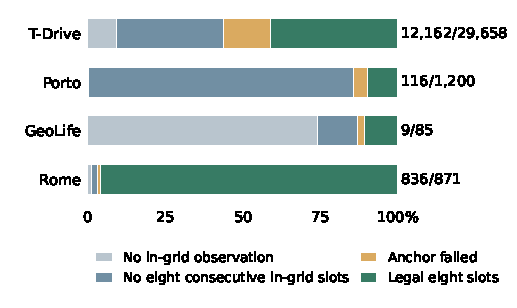
\includegraphics[width=\columnwidth]{figures/submission_four_corpus_20261030.pdf}
\caption{Offline input-screen outcomes across three observed actor-day frames per corpus.}
\label{fig:real-trace-impact}
\end{figure}

Individual legality and a complete simultaneous input are distinct. Of 15 predetermined Rome rosters per size, 11 at N=8 and two at N=32 have individually legal histories for every member, but none of these has a common start, giving 0/11 and 0/2. At N=100 no roster is individually all-legal and the conditional result is undefined.

\subsection{Compact Semantic Binding}
\label{sec:eval-accepted-history-deployment}
\label{sec:eval-binding}
\label{sec:eval-dense}

The masked-moment check rejects a native-valid report for cell 42 when the
hidden proof authorizes cell 2312. The authority records no commit, head
advance or quota consumption. This exercises Lemma~\ref{lem:native-moment-fidelity} on native-valid inputs.

At 10,001 bins, the standalone masked-moment module has 5,779 constraints versus 79,002,390 for direct seed binding, a 13,670.60$\times$ ratio (Figure~\ref{fig:binding-circuit-cost}). The complete transition measurements in Table~\ref{tab:binding-cost} concern different relations and fixed fixtures, rather than the same business input. Setup verification preceded measurement. The five paired fullProve time ratios have median 89.73, quantifying component costs for these implementations. fullProve includes witness generation. Native moment evaluation scans the vector in \(O(D)\), and the compact relation relies on native one-hot validity.

\begin{table}[t]
\centering
\caption{Fixed-fixture transition component costs across five interleaved pairs.}
\label{tab:binding-cost}
\footnotesize
\setlength{\tabcolsep}{3pt}
\begin{tabular*}{\columnwidth}{@{\extracolsep{\fill}}lrr@{}}
\toprule
Metric & Masked moment & Vector commitment \\
\midrule
fullProve median (s) & 3.4805 & 311.8310 \\
fullProve range (s) & 3.4674--3.4820 & 311.5520--312.4485 \\
Prove CPU median (s) & 3.4748 & 311.3832 \\
Process peak RSS median (GiB) & 0.2977 & 13.8623 \\
Internal verify median (s) & 0.03230 & 0.04054 \\
\bottomrule
\end{tabular*}
\end{table}

\begin{figure}[t]
\centering
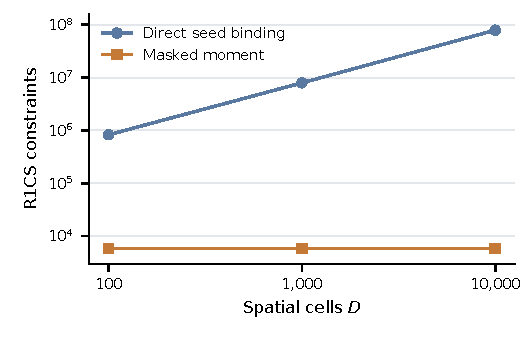
\includegraphics[width=\columnwidth]{figures/submission_binding.pdf}
\caption{Standalone binding circuit R1CS sizes across histogram widths.}
\label{fig:binding-circuit-cost}
\end{figure}

\subsection{Feedback and First Exposure}
\label{sec:eval-origin-feedback}
Origin checks protect an earlier boundary. In the feedback control,
disabling body-owner signature and authority-certificate checks allows
copied honest reports with known masks to produce receipts that reveal
index 4237. Later admission refusal does not erase this observation.
The complete guard refuses the same input before decryption and receipt
feedback. Normal reports and exact retries continue through the protected
path. The result locates origin authentication before receipt feedback.

\label{sec:eval-ladder}
\label{sec:eval-dap-control}

\label{sec:eval-gate-position}
\label{sec:eval-selection-recovery}

Two legal histories produce the same complete eight-owner histogram but
produce different seven-owner subset outputs (Figure~\ref{fig:cohort-exposure}).
The native subset control exposes a difference of two counts in unnormalized
L1, the sum of absolute bucket-count differences. SHTPC refuses the incomplete set before an honest share is exposed,
illustrating the first-exposure boundary in
Proposition~\ref{prop:exposure-separation}.

\begin{figure}[t]
\centering
\begin{minipage}[t]{0.485\columnwidth}
\centering
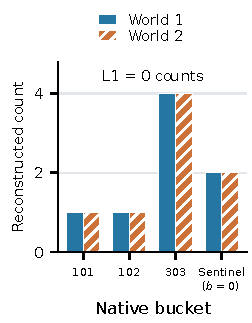
\includegraphics[width=\linewidth]{figures/submission_exposure_a.pdf}\par
{\footnotesize (a)}
\end{minipage}\hfill
\begin{minipage}[t]{0.485\columnwidth}
\centering
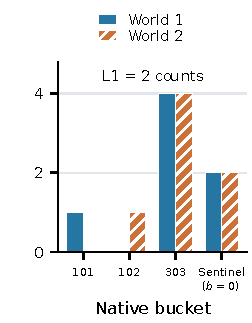
\includegraphics[width=\linewidth]{figures/submission_exposure_b.pdf}\par
{\footnotesize (b)}
\end{minipage}
\caption{Native outputs for (a) the complete eight-member cohort and (b) its seven-member subset.}
\label{fig:cohort-exposure}
\end{figure}

\label{sec:strong-baselines}
The external controls use different aggregation interfaces. A SCIF
acceptance bridge detects omitted positives, eligible zeros and equal-count
substitutions only after trusted output reconstruction, because that output
carries no external member evidence~\cite{Su2025SCIF}. A PEAR role run
reconstructs an exact eight-report, 10,001-bin output and rejects invalid
inputs without supplying SHTPC's current predecessor or accepted-set
reference~\cite{Acharya2025PEAR}. These controls complement rather than
replace the native first-exposure check.

\subsection{History Recovery}
\label{sec:eval-failure-cuts}

In the 100-user campaign, redelivery after one or ten withheld accepted
decisions restores all 100 eligible members and the exact 10,001-coordinate
output. The campaign fixes 700 transitions. Affected services restart on their
retained databases while the key-holding controller remains live.
Table~\ref{tab:complete-history-functional} summarizes the observed obligations.

\begin{table}[t]
\centering
\caption{Native validation of security obligations.}
\label{tab:complete-history-functional}
\label{tab:failure-cuts}
\footnotesize
\begin{tabularx}{\columnwidth}{@{}lYY@{}}
\toprule
Obligation & Security boundary & Observed outcome \\
\midrule
P1 & Output binding & 2312/42 mismatch rejected, no commit \\
P2 & Feedback isolation & Guard-off revealed 4237, guard-on blocked \\
P3 & Atomic history & Conflicting successor rejected, retry idempotent \\
P4 & Complete exposure & Missing 1 or 10 blocked, 100-member output restored \\
P4 & Subset exposure & Distinguishable seven-of-eight subset blocked \\
\bottomrule
\end{tabularx}
\end{table}

A two-owner native trace combines sequential competing registration, retries
and selective delivery. The conflicting successor is refused, and redelivery
restores the frozen set and exact output. The run passes seven driver and 469
independent semantic checks. Separate recovery tests cover concurrent
preparation, changed peer bytes, arranged commit-first and freeze-first SQL
orders, and failure paths that retain accepted state.

\label{sec:eval-model-check}
TLA+/TLC 2.19 checks 41 configurations of ClosureV5: fixtures have one to
three owners and reports, two roles, and one or two windows. The artifact's
\path{current/model/cases.json} fixes each case's bounds; its specification
is \path{current/model/ClosureV5.tla}. Six safety and one fair-progress configurations pass;
guard removals expose invariant violations, and reachability and temporal
controls exercise witnesses and fairness assumptions.


\subsection{Cost of the Enforced Contract}
\label{sec:eval-architecture}
\label{sec:eval-certification}
\label{sec:eval-performance}
\label{sec:eval-native}

Figure~\ref{fig:mechanism-cost} reports four mechanism configurations for
100 eligible reports. The two Full server-window observations are 770.39~s
and 824.36~s. Shared registration, lock, exposure and collection mean the
configurations do not isolate additive increments or P4. M/A/Z have three runs and Full has two, with median lines in the figure. The separate Prio3
native-component reference has a 10.59~s median at a different endpoint.

\begin{figure}[t]
    \centering
    \begin{minipage}[t]{0.48\columnwidth}
        \centering
        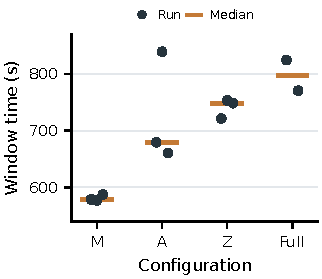
\includegraphics[width=\linewidth]{figures/submission_mechanism_a.pdf}
        \par\vspace{2pt}
        {\footnotesize (a)}
    \end{minipage}
    \hfill
    \begin{minipage}[t]{0.48\columnwidth}
        \centering
        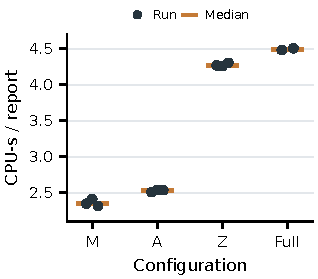
\includegraphics[width=\linewidth]{figures/submission_mechanism_b.pdf}
        \par\vspace{2pt}
        {\footnotesize (b)}
    \end{minipage}

    \caption{Mechanism costs for 100 eligible reports, with (a) server-window wall time and (b) server CPU per report.}
    \label{fig:mechanism-cost}
\end{figure}

Prio3 supplies native validity and aggregation. M adds masked-moment consistency, A adds permit and receipt authorization, quota and durable delivery, and Z proves the hidden transition. Full combines these mechanisms with atomic admission and complete first-exposure reservation. In a separate server-only diagnostic, admission and verification account for the largest measured CPU category.

\paragraph{Full lifecycle and trusted generation.}
Table~\ref{tab:session-cost} reports selected phase and session costs for the Full/T pair. Full takes 72.37 minutes for the session and 8.82 minutes for the eligible window, compared with 52.86 and 6.31 minutes under T. These single observations are lower under T by 26.96\% and 28.54\%, respectively, under a different trust boundary. Full does not disclose coordinates to the trusted generator. T omits transition proofs and moments but retains 100 genesis proofs. The window includes collection, which takes 57.062 s for Full and 65.326 s for T. The listed phases do not exhaust the session.

\begin{table}[t]
\centering
\caption{Selected phase and session costs for the Full and trusted-generation pair.}
\label{tab:session-cost}
\footnotesize
\begin{tabular}{@{}lrr@{}}
\toprule
Phase & Full (s) & Trusted generation (s) \\
\midrule
Setup and genesis & 197.225 & 201.259 \\
600 history priming & 3322.162 & 2309.288 \\
Eligible window (100 reports) & 529.450 & 378.330 \\
Total session & 4342.151 & 3171.444 \\
\bottomrule
\end{tabular}
\end{table}

\section{Related Work}
\label{sec:related-work-summary}

Table~\ref{tab:related-comparison} compares the guarantees and integration
obligations most relevant to accepted-history closure.


\begin{table*}[b]
\centering
\caption{Related guarantees and their connection to accepted-history closure. The last column identifies integration obligations, not attacks or missing guarantees under another protocol's model.}
\label{tab:related-comparison}
\footnotesize
\setlength{\tabcolsep}{3pt}
\begin{tabularx}{\textwidth}{@{}>{\raggedright\arraybackslash}p{.20\textwidth}YY@{}}
\toprule
Representative work & Established focus & Connection to this contract \\
\midrule
Prio, ACORN, EIFFeL~\cite{Corrigan2017Prio,Bell2023ACORN,Chowdhury2022EIFFeL} & Validity of private inputs & Bind the certified transition to actual retained outputs \\
SCIF, PEAR~\cite{Su2025SCIF,Acharya2025PEAR} & Inclusion or verifiable aggregation under their trust models & Use the external accepted set before first exposure \\
Stateful aggregation, PCD~\cite{Ball2024Stateful,Chiesa2010PCD} & Private aggregate state or evidence of computation history & Authorize the current per-identity head and atomic advancement \\
PrivStats, ZKLP~\cite{Popa2011PrivStats,Ernstberger2025ZKLP} & Upload accountability or hidden location predicates & Connect accepted history, retained output and release membership \\
SecAgg, Flamingo~\cite{Bonawitz2017SecureAggregation,Ma2023Flamingo} & Secure aggregation, dropout or multiple rounds & Preserve a complete prelocked cohort at first exposure \\
DP heatmaps, Prochlo~\cite{Bagdasaryan2022SparseHeatmaps,Bittau2017Prochlo} & Output privacy or shuffled analytics & Supply an admitted-history input to the chosen release mechanism \\
SHTPC & Accepted-history closure & P1--P4 with correct services and separate single-cohort privacy \\
\bottomrule
\end{tabularx}
\end{table*}

\paragraph{Validation and inclusion}
Prio+, VDAFs and DAP separate private input validation from aggregation and
collection~\cite{Addanki2022PrioPlus,Barnes2023VDAF08,Geoghegan2026DAP,Davis2023VDAFPrivacy}.
Poplar, Mastic and Whisper extend private analytics to heavy hitters, weighted
metrics and streams~\cite{Boneh2021Poplar,Mouris2025Mastic,Rathee2024Whisper}.
ELSA and RoFL address malicious contributions, while fully linear PCPs enable
proofs on shared data~\cite{Rathee2023ELSA,Lycklama2023RoFL,Boneh2019FullyLinear}.
VerSA and VeriFL study aggregate verification, with later analyses and
repairs~\cite{Hahn2023VerSA,Luo2024VerSAComments,Guo2021VeriFL,Guo2022VeriFLFix}.
Input validity constrains the reconstructed value, whereas inclusion constrains
which reports participate. SCIF supplies honest-input inclusion under its
server-corruption threshold. PEAR can express an application predicate, but
using that predicate with evolving state also requires an authenticated current
predecessor and atomic advancement. SHTPC connects these interfaces to an
external accepted history before the first honest share becomes decryptable.
In particular, matching counts or histogram values do not certify inclusion of
an eligible zero-bit record.

\paragraph{State and authorization}
Proof-carrying data and recursive composition propagate evidence of computation
history~\cite{Chiesa2010PCD,Bitansky2012Recursive}. Privacy Pass, DAP report
authentication, zk-creds and ZEBRA support authorization or private credential
claims~\cite{Davidson2024PrivacyPass,Priebe2023ReportAuth,Rosenberg2023ZKCreds,Rathee2022Zebra}.
VPriv and PrETP connect private locations to charges~\cite{Popa2009VPriv,Balasch2010PrETP}.
PrivStats combines anonymous reporting with per-point and total upload quotas
and sample-range proofs. Its accountability goal is therefore closer to this
work than origin authentication alone. SHTPC additionally authorizes a successor
against the actual per-identity head and binds its retained contribution to
complete first exposure. A transition proof can remain valid after another
successor commits, so checking that proof and updating the head are distinct
operations. SecAgg+ and LightSecAgg address dropout recovery~\cite{Bell2020SecAggPlus,So2022LightSecAgg};
SHTPC instead preserves its prelocked membership through durable redelivery.

\paragraph{Output privacy}
RAPPOR randomizes locally, while Prochlo separates encoding, shuffling and
analysis~\cite{Erlingsson2014RAPPOR,Bittau2017Prochlo}. Shuffle-model analyses
quantify amplification from anonymous randomized reports~\cite{Cheu2019distributed,Erlingsson2019Amplification,Balle2019privacy}.
Differential privacy protects released statistics~\cite{Dwork2006calibrating,Dwork2014algorithmic},
while geo-indistinguishability and temporal models address location disclosure
and correlation~\cite{Andres2013geoi,Xiao2015Temporal,Montjoye2013Unique}.
Sparse heatmaps combine secure aggregation with distributed differential
privacy, separating private computation from information in the released
statistic. These goals complement SHTPC's guarantee that the statistic contains
the admitted claims. Applying an output mechanism requires its own sensitivity,
release policy and composition analysis, including which party can first
decrypt an exact result. Its single-cohort simulation bounds additional protocol
information under the declared output and metadata, rather than inference
from successive released heatmaps.

\clearpage
\section{Discussion and Conclusion}
\label{sec:limitations}
\label{sec:conclusion}

This section discusses the deployment tradeoffs and limits of SHTPC.

\paragraph{Deployment tradeoffs.}

Periodic reporting makes a fixed release reference useful when complete
cohort statistics take priority over immediate subset availability. One internally inconsistent body or vanished predeclared member
can hold the cohort, while durable delivery handles later transport failures.
This tradeoff suits applications that value a complete declared cohort or
explicit refusal over immediate partial statistics. Input coverage and a common start affect whether a prelocked complete set is available. The measured Full session includes six history-initialization steps, whose cost can be weighed against subsequent window scheduling.

The compact relation uses native Histogram validity, while native processing
still scans the vector in \(O(D)\). Other input domains require their own
identifying relation and privacy analysis.

\paragraph{Output privacy.}

Public activity and contribution bits remain visible, and a Collector who knows every other owner's cell can infer the remaining contribution from an exact total. The stated single-cohort privacy model protects the additional protocol views. Differential privacy for the output and composition across multiple releases require separate mechanisms and analysis.

SHTPC connects hidden-state authorization to the contributions retained by native private aggregation and to complete-cohort first exposure. Masked moments, atomic admission and durable reservation connect these boundaries under the stated service and trust assumptions. Native attack and recovery tests exercise the interfaces, while component and lifecycle measurements characterize their costs and the input screen distinguishes individual legality from simultaneous complete input.


\section{Artifact Availability}
\label{sec:artifact}
The repository at
\url{https://anonymous.4open.science/r/semantic-closure-artifact-2300/updates/2026-10-29/}
contains the manuscript, component sources and evidence map.
\label{sec:artifact-proofs}
Its \nolinkurl{proof/README.md} maps the numbered G4b proof documents to the
statements here. G4b 02 is
\nolinkurl{proof/02-groth16-extraction-and-budget.md}.
G4b 03, 04 and 07 contain the native query ledger, full-view online simulation
and ordered composition hybrids. The directory also includes their explicit
budget contracts and version provenance. These detailed arguments use the
stated three-key source model. Raw trajectories follow their original licenses.

\FloatBarrier
\clearpage
\label{boundary:references}
{\footnotesize
\printbibliography}
\clearpage
\appendices
\section{Interface, Policy and Composition Details}
\label{boundary:appendix}
\label{sec:composition-failures}

\paragraph{Interface and policy.}
\label{cor:submission-shared-tag}
An independent acceptance rectangle with valid pairs for two primaries also
contains their mismatched cross-spliced pair. Thus every rectangle contained in
the same-primary relation has one primary.
\label{sec:history-interface}
For complete legal and illegal views \(X_0,X_1\), let
\(a_i=\Pr[V(X_i)=1]\). Completeness and soundness errors satisfy
\(e_c+e_s=1-a_0+a_1\ge1-|a_0-a_1|\), which is one for identical views.

\label{app:policy}
For real-trace replay, local equirectangular projection uses radius
6,371,000\,m and centers (116.4, 39.9) for T-Drive and GeoLife, (-8.61, 41.15) for Porto, and (12.4964, 41.9028) for Rome. Coordinates are shifted by 5,000\,m and floored to integer meters.
Points outside [0, 9999] in either coordinate are excluded from legal histories.
The earliest observation per 300-second slot is used without gap filling.
Pressure histories require eight consecutive occupied slots and, for Porto,
one trip. The screen uses \(K=6\), a 40 m/s speed tier and a 3,300\,m anchor cap. The four-corpus screen uses the same slots, grid and policy, with corpus-specific parsers and trip or trajectory boundaries. Rome uses a cleaned raw-point cache with valid coordinates, a city bounding box and duplicate timestamps removed. Its date labels follow the original naive wall-clock calendar. Each corpus uses three frozen dates. GeoLife and Rome dates were selected by observed actor coverage before legality screening.

The hidden ADWC relation bounds squared displacement from the accepted
predecessor by \(\tau_u^2\Delta t_t^2\), and from the anchor
\(\mathbf a_t=\mathbf x_{\max(0,t-K)}\) by
\(\min\{\tau_u^2(\Delta T_t^{(K)})^2,c_{\rm policy}^2\}\), with speed tier
\(\tau_u\), anchor cap \(c_{\rm policy}\) and
\(\Delta T_t^{(K)}=K\Delta t_{\rm slot}\). Enrollment proves a hidden
genesis. The first \(\max(K,2)\) accepted steps advance history without
aggregation eligibility, and the authority checks the proof's commitment
references against actual accepted history. Accepted steps, slots,
timestamps and revisions are distinct.

\label{app:exposure-separation}
Swap two owners' positive cells in metadata-compatible legal worlds.
Complete aggregates coincide. A batch containing one swapped owner has
different aggregates, so the corrupted role and Collector distinguish when
the honest share arrives. A subsequent publication refusal cannot erase it.
This proves Proposition~\ref{prop:exposure-separation}.

\label{app:closure-proof}
Registration stores full signed candidates without advancing history. Lock fixes
\(P_w,R_w\) before private processing, and permits reference only actual committed
predecessors and anchors. Commit atomically checks head and quota and records
the successor, history and signed decision. This linearization point enables
exactly the next transition in Definition~\ref{def:legal-history} and
preserves real-time precedence. Apply changes \(N_{S,w}(r)\) from zero to one
only for eligible commits, with duplicate retries as no-ops. Reserve checks
the registration projections in Eq.~\eqref{eq:final-report-set} and all record links, then stores an
immutable selector and sum before send. Recovery preserves reservations;
pre-exposure abort retains partial commits and post-send failure retains the
exposed snapshot. Induction gives Eq.~\eqref{eq:export-safety} at every
prefix, and native fidelity gives Eq.~\eqref{eq:closure-release}.

\section{Joint Privacy and Concrete Bounds}
\label{app:native-theory}

\begin{table*}[t]
\centering
\caption{Adjacent hybrids and their loss; \(N\) counts honest native sources
and \(Q_i\) the seven stream budgets.}
\label{tab:hybrid-ledger}
\footnotesize
\begin{tabularx}{\textwidth}{@{}clYr@{}}
\toprule
Step & Change and simulator knowledge & Loss \\
\midrule
1 & Nonce deduplication over public unprepared sources & \(N^2/2^{128}\) \\
2 & Initial usage, seed and binder programming & \(N[Q_4+2(Q_3+Q_6+Q_7)+Q_5]/2^{128}\) \\
3 & Share and part programming with corrupt shares fixed & \(N[Q_1+Q_2+2Q_7]/2^{128}\) \\
4 & Prover-coin removal for unexposed seeds & \(NQ_4/2^{128}\) \\
5 & Source simulation, full verifier, joint receipts, raw trace and first exposure & \(0\) \\
6 & Strict-time truncation after \(L+128\) candidates & \(t_N\) \\
\bottomrule
\end{tabularx}
\end{table*}

\phantomsection
\paragraph{Trust and lifecycle.}
\label{app:trust-lifecycle}
Clients hold report-signing keys, admission holds enrollment and authorization
keys, and each role holds input HPKE and receipt keys. The shared native
verification key is uniform in \(\{0,1\}^{128}\) and hidden from clients in
the integrity game. Only the Collector holds the aggregate HPKE secret.
Finalizer uses authenticated admission records, and Decoder uses the decryption
result and public verification keys.

Registration is authenticated and confidential. Bodies, permits, commits and
receipts authenticate owner, task, window and context. Inputs and sidecars use
recipient-bound labeled HPKE. Shares use the Collector key with context and
set checks. Collector-to-Decoder delivery authenticates the finalized-set
certificate. Preparation uses durable journals and leases. Transport may
delay, drop or replay messages. Privacy includes observer messages under \(\mu\).

Credential epochs bind signed context while identity and quota survive rotation.
Revocation, post-compromise recovery and forward secrecy are outside the model.
Corrupted role state is included, honest role secrets and backups are not.
Durability requires retention through replay checks and recovery.

\phantomsection
\label{app:native-interface}
BabyJubJub Pedersen commitments~\cite{Pedersen1991Commitment} use canonical
prime-order points, fixed public bases and uniform full-domain blinders.
The hidden genesis and transition relations bind the true predecessor and
\(K\)-anchor. With native field
\(q=2^{128}-7\cdot2^{66}+1\), canonical \(r_A,r_R,T\in[0,q-1]\)
and \(x\in[0,D]\), where \(D<q\), give
\(0\le x+r_A+r_R<3q\). The carry \(\chi\in\{0,1,2\}\) therefore
makes \(x+r_A+r_R=T+\chi q\) an integer equality. Both sides are below
\(3q<2^{130}<p_{\rm proof}\), where the BN254 scalar modulus satisfies
\(2^{253}<p_{\rm proof}<2^{254}\). Thus equality in the proof field
cannot wrap. Successful counts fit a signed 64-bit integer,
so reconstructed histograms do not wrap modulo \(q\).

\begin{lemma}[Origin isolation]
\label{lem:origin-isolation}
Outside authentication, digest and origin-allocation failures, a protected
ciphertext enters private processing only in its registered source body.
\end{lemma}
\begin{proof}
Allocation binds the identifier to its owner before publication. The complete
body, encryption labels, installed lock and process permit fix the input before
decryption. A transplant changes authenticated bytes or requires an already
allocated identifier. Exact retries reuse the source and durable native state.
\end{proof}

\phantomsection
\label{app:primitive-reductions}
Fix finite budgets before the challenge. All counts include honest
construction, rejected inputs, offline queries, retries and rolled-back work.
For the three-key basis of Lemma~\ref{lem:related-crs-extraction}, let
\(S=S_g+S_t+S_l\) count fresh external real or simulated source proofs and
\(V=V_g+V_t+V_l\) count verifications under the three keys. The \(Q_{G_1},
Q_{G_2},Q_{G_T},Q_{\rm pair}\) budgets count typed group-oracle outputs
beyond the separately counted sources, imports and verifications. The counts
\(I_1,I_2\) cover source-group imports, and native XOF queries \(Q_i\) use a
separate budget. The proof-field ledger is
\begin{align}
 h_1={}&330974+2S+Q_{G_1}+I_1\notag\\
       &+13V_g+53V_t+13V_l,\notag\\
 h_2={}&80986+S+Q_{G_2}+I_2+V,\notag\\
 h_T={}&5+Q_{\rm pair}+Q_{G_T}+7V,\notag\\
 d_G={}&32769\tbinom{h_1}{2}+16383\tbinom{h_2}{2}
       +49152\tbinom{h_T}{2},\notag\\
 g_{\rm coll}={}&\min\{1,d_G/(p_{\rm proof}-16385)\},\notag\\
 g_{\rm aff}={}&\min\{1,S(3p_{\rm proof}-2)/p_{\rm proof}^2\},\notag\\
 g={}&\min\{1,g_{\rm setup}+g_{\rm coll}+g_{\rm aff}\}.
 \label{eq:groth-budget}
\end{align}
The \(h\) values bound group handles at one hybrid endpoint. Sampling directly
from the specified good setup domain gives \(g_{\rm setup}=0\). Unknown
trapdoors and independent setup entropy remain premises. The affine term is a
conservative additional charge that can overlap the collision event. The fixed
source inventory and derivation appear in artifact document G4b 02,
Sections 2--7 (Section~\ref{sec:artifact-proofs}).

Let \(Q_i\) count native stream queries by domain, in order measurement,
proof share, joint randomness, prover randomness, query randomness, joint
seed and joint part. Put \(Q=\sum_{i=1}^{7}Q_i\), and let \(P_{\rm att}\)
count distinct attack preparation inputs. The actual public key tag is a
96-bit prefix of the verification-key hash. For \(G_5\) external candidate-key
queries, let \(K\) be the uniform 128-bit key and \(Z=f(K)\) its tag.
On the no-hit branch, each tag value determines at most \(G_5\) candidate
keys \(E_z\). Averaging over tags gives
\[
 \Pr[K\in E_Z]=2^{-128}\sum_z|f^{-1}(z)\cap E_z|
 \le 2^{96}G_5/2^{128}.
\]
Thus \(\kappa_{\rm tag}\le\min\{1,G_5/2^{32}\}\), without assuming
uniform tag fibers. The factor two below charges the two secret-key
replacement hybrids, each with one such first-hit event.
An additional SHA256 one-wayness assumption on uniform 128-bit inputs gives
the alternative bound \(\kappa_{\rm tag}\le a_{\rm OW128}\).
Scanning all queried keys gives that reduction with one additional hash per
candidate. Collision resistance alone does not supply this assumption.
The native validity term is
\begin{equation}
 \begin{split}
 v_N=\min\bigl\{1,{}&10256(Q+P_{\rm att})/q+2\kappa_{\rm tag}\\
                   &+(2P_{\rm att}+Q)^2/2^{128}\bigr\}.
 \end{split}
 \label{eq:native-validity-bound}
\end{equation}
Here \(10256=10002+254\). For 10,001 bins the invalid-input identity
has error at most \((10001+1)/q\), while a false gadget polynomial of
degree at most 254 contributes \(254/q\). The root-abort branch remains
in the experiment. This term concerns invalid-input acceptance. Privacy against a corrupted
role, which already knows the verification key, has a separate nonce-based
bound below.

\begin{definition}[Exposure equivalence]
\label{def:exposure-equivalence}
Using the declared indices of Definition~\ref{game:privacy}, legal histories
with common public structure \(\mu\) are exposure-equivalent for \(R_w\) when
\begin{equation}
 \sum_{i\in R_w}\mathbf e_{y_i^{(0)}}=
 \sum_{i\in R_w}\mathbf e_{y_i^{(1)}}.
 \label{eq:exposure-equivalence}
\end{equation}
Authority-only has no aggregate query and does not require this equality.
\end{definition}

\begin{proposition}[Effect of the exposure family]
\label{prop:exposure-family}
A fixed full cohort permits histogram-preserving reassignment. If every
size-\(k\) subset can instead be exposed, \(1\le k<n\), equal sums on
all such subsets force identical per-record native indices.
\end{proposition}
\begin{proof}
Set \(d_i=\mathbf e_{y_i^{(0)}}-\mathbf e_{y_i^{(1)}}\).
Exchanging \(i,j\) in a size-\(k\) subset gives \(d_i=d_j\).
A size-\(k\) sum then gives \(kd_i=0\), hence \(d_i=0\) over integers.
\end{proof}

\label{lem:pedersen-language-lifting}
Full-domain blinding lets every hidden state point represent any fixed legal
reference history. History-node aliases reuse the same point. This is
language membership for the proof hybrid, not an extraction algorithm.
\label{lem:receipt-coupling}
Equation~\eqref{eq:receipt-simulation} gives the joint receipt law
\((T,m_h)=(U,U-F(v_c^{\rm orig})-r_c)\). For authority-only,
uniform \(T,U\) give \((T,m_A,m_R)=(T,U,T-U)\).

The native model is a domain-separated programmable random oracle indexed by
usage, seed, complete binders and raw offset. Repeated descriptors reuse rejected
candidates and unconsumed prefetch too. Applying these bounds to the concrete
TurboSHAKE128 XOF requires this idealization beyond XOF pseudorandomness.
The native kernel specializes the two-party, single-proof analysis in the
2024-09-25 revised full version of \cite{Davis2023VDAFPrivacy} to the
pinned Histogram interface. The following bounds and simulator account for
this interface and its differences rather than directly copying the old bound.

\begin{lemma}[Concrete Histogram preparation view]
\label{lem:concrete-histogram-view}
The two-role, single-proof 10,001-bin Histogram has a 455-element proof,
202-element verifier and 128 interpolation points \(\Omega\).
For valid inputs and query \(t\notin\Omega\), its full verifier is
\((0,W_0,\ldots,W_{199},\sum_{j=0}^{99}W_{2j}W_{2j+1})\), with
independent uniform \(W_i\). Queries in \(\Omega\) take the same root-abort
branch in both worlds.
\end{lemma}
\begin{proof}
Each valid-input wire has nonzero random-value coefficient
\((t^{128}-1)/(128(t-1))\). Its affine inverse makes evaluations
independent uniform \(W_i\), determining the gadget coordinate.
For \(t\in\Omega\) both worlds abort identically.
\end{proof}



\begin{theorem}[Concrete two-party native privacy]
\label{thm:concrete-two-party-native}
In this programmable-oracle model, let \(N\) count honest native source
reports, including unprepared reports.
A single-world native stream simulation has loss at most
\begin{align}
 Q_*&=Q_1+Q_2+Q_5+2(Q_3+Q_4+Q_6)+4Q_7,\notag\\
 b_N&=\min\{1,(N^2+NQ_*)/2^{128}\}.
 \label{eq:native-stream-bound}
\end{align}
Before exposure the simulator uses no aggregate query. At exposure it uses
one complete-cohort query under Eq.~\eqref{eq:exposure-equivalence}.
\end{theorem}
\begin{proof}[Proof sketch]
Couple corrupt inputs and program fresh domain-separated streams. Nonce
collisions and prior queries give Eq.~\eqref{eq:native-stream-bound}.
For either corrupt role, fix its original measurement/proof shares, key and
nonce. Sample full verifier \(\Sigma\) from the lemma, compute the corrupt original
distributed query \(z_c^{\rm orig}\), and set \(z_h=\Sigma-z_c^{\rm orig}\).
Each active response \(z'_c\) undergoes \(\mathsf{Decide}(z_h+z'_c)\) and
seed-equality checks. Root queries reuse the abort branch. Helper exact retries
reuse journaled bytes. Leader uncommitted recomputations use the same
\(\Sigma,z_h\) and original state for changing responses, committing at most
once. Verdicts and modeled times follow this state without real-verdict/time
oracles. Recomputed work remains budgeted. G4b 03, Sections 3--7, and 04,
Sections 2--7, give the descriptors and full online hybrids in the
artifact (Section~\ref{sec:artifact-proofs}).
\end{proof}

\begin{theorem}[Joint privacy of admission and native release]
\label{thm:native-single-batch-privacy}
Use the privacy experiment of Definition~\ref{game:privacy}, the source and
programmable-oracle models above, and their primitive bounds.
Let \(X\) denote authority-only, active-role-and-Collector, or that
aggregation view with the authority's business view. Let \(g\) be the bound
in Eq.~\eqref{eq:groth-budget}, \(\epsilon_H\) the full-digest SHA256 collision
advantage over all hash queries and bytes, \(a_X\) the sum of signature
EUF-CMA advantages for correct-party keys unknown to the
observer, and \(c_B\) the five-purpose Pedersen binding advantage. Let
\(N_{\rm id}\) count honest identifier draws, including failed reservations,
and \(G_{\rm id}\) count adversarial guesses before publication. With \(C_X\)
hidden HPKE encapsulations, let \(H_X\) sum their labeled IND-CCA advantages and set
\begin{align}
 B_X&=\min\{1,g+\epsilon_H+a_X+c_B+N_{\rm id}G_{\rm id}/2^{128}\},
 \label{eq:route-bound}\\
 e_X&=\min\{1,2(C_X+10)B_X+H_X+b_N+t_N\},\\
 \operatorname{Adv}_X&\le\min\{1,2e_X\},
 \label{eq:native-joint-bound}
\end{align}
where \(t_N\le\min\{1,5N\binom{10129}{129}\rho^{129}\}\) and
\(\rho=(2^{128}-q)/2^{128}\). Authority-only needs no aggregate equality.
The other two views require Eq.~\eqref{eq:exposure-equivalence}.
\end{theorem}
\begin{proof}[Hybrid outline]
Rows 1--4 of Table~\ref{tab:hybrid-ledger} sum to the bound in
Eq.~\eqref{eq:native-stream-bound}. The \(C_X\) labeled HPKE hops and ten
macro hops each have two endpoints, each charged \(B_X\). Their endpoint
charges give \(2(C_X+10)B_X\), while \(H_X\) adds one IND-CCA advantage per
hidden encapsulation. The ten macro hops cover source proofs, nonce
deduplication, initial oracle programming, shares and parts, prover coins,
the full verifier, points and receipts, raw traces, business and exposure
processing, and truncation. Artifact document G4b 07, Section 5, gives
the ordered ledger (Section~\ref{sec:artifact-proofs}).
The five field streams are measurement, proof share, joint,
prover and query randomness. Seed and part streams output bytes. A retry
preserves native randomness and original-source state, including the report,
key, nonce and original shares. Active responses and verdicts can vary.
Truncation after
\(L+128\) candidates requires 129 rejections to fail. A union bound over
\(5N\) streams with \(L\le10001\) gives \(t_N\). Repeated descriptors
reuse their stream. The two histories share one ideal view, so their distances
add.
\end{proof}
For aggregation views, \(C_X\le2N\) counts one hidden native input and one
sidecar for the honest role per honest source. Authority-only has both roles'
inputs and sidecars, so \(C_X\le4N+E_{\rm enc}\), where \(E_{\rm enc}\) counts
fresh aggregate encapsulations visible to the authority, including re-encrypted
retries. Each term in \(H_X\) uses one challenge and its recipient-key-specific
time, permitted decryption-query count and byte budgets. Primitive time
budgets include the reduction's work. For integrity, the
corresponding \(X=C\) route bound is \(B_C\). Malicious
sources use authorized decryption and real native execution. Equation~\eqref{eq:simulated-honest-export}
subtracts their declared indices and adds their actual honest-role outputs.


\begin{lemma}[Export refinement]
\label{lem:export-refinement}
On the legal reachable install domain, the optimized export transaction
accepts the same reservations and payload bindings as the full-scan
transaction.
\end{lemma}
\begin{proof}
Unique unsigned-decimal window text selects the same reference row. For
integer-only records, fixed JSON ordering/escaping and unique integer text make
canonical and parsed equality equivalent. Floats are excluded. Other records
use parsed comparison. The projection retains body, window, record and lock
identifiers and reads complete records and the lock certificate from the reference.
Both transactions check the same freeze, lock, count, commit, eligible retained-link,
consumed membership, frozen-set, reservation and payload conditions under one control
lock and repeatable-read snapshot. Locking one complete \(P\) keeps the reference consistent. Install rejects
rows outside this domain.
\end{proof}

\end{document}
